\documentclass[aspectratio=169]{beamer}

\usetheme{Madrid}
\usecolortheme{seahorse}
\setbeamertemplate{navigation symbols}{}
\setbeamertemplate{footline}[frame number]

\usepackage{graphicx}
\usepackage{tikz}
\usetikzlibrary{shapes,arrows,positioning,fit,backgrounds}
\usepackage{booktabs}
\usepackage{xcolor}
% enumitem not used - conflicts with beamer

\definecolor{mainblue}{RGB}{0,83,156}
\definecolor{lightblue}{RGB}{200,220,240}
\definecolor{darkgray}{RGB}{60,60,60}
\definecolor{successgreen}{RGB}{34,139,34}
\definecolor{warnorange}{RGB}{255,140,0}
\definecolor{alertred}{RGB}{178,34,34}

\setbeamercolor{title}{fg=mainblue}
\setbeamercolor{frametitle}{fg=mainblue}
\setbeamercolor{structure}{fg=mainblue}

\title{Adaptive Hierarchical Planning with Failure Detection and Strategy Switching}
\subtitle{for LLM-Based Agents}
\author{Mudit Baid}
\institute{Stanford University \\ CS 372}
\date{Winter 2026}

\begin{document}

% ============================================================
% TITLE
% ============================================================
\begin{frame}
\titlepage
\end{frame}

\begin{frame}{Outline}
\tableofcontents
\end{frame}

% ============================================================
\section{Problem Statement}
% ============================================================

\begin{frame}{LLMs as Planners: Three Key Limitations}

\begin{columns}[T]
\begin{column}{0.55\textwidth}

\textbf{1. No hierarchy}
\begin{itemize}
    \item Plans are flat action sequences
    \item No distinction between goals and actions
    \item Early errors propagate unchecked
\end{itemize}

\vspace{0.3cm}
\textbf{2. No strategy adaptation}
\begin{itemize}
    \item Same prompting for spatial, logical, procedural subtasks
    \item CoT, ToT, ReAct each have strengths---none adapts
\end{itemize}

\vspace{0.3cm}
\textbf{3. No failure recovery}
\begin{itemize}
    \item Plan fails midway $\rightarrow$ restart from scratch
    \item Prior progress is discarded
\end{itemize}
\end{column}

\begin{column}{0.4\textwidth}
\centering
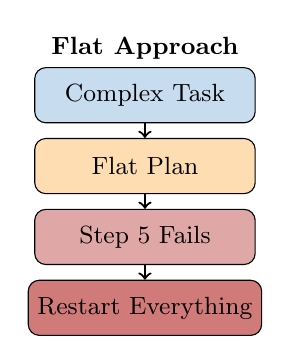
\begin{tikzpicture}[scale=0.75]
    % Flat approach
    \node[font=\small\bfseries] at (0,4.2) {Flat Approach};
    \node[draw, rounded corners, fill=lightblue, minimum width=2.8cm, minimum height=0.7cm, font=\small] (task) at (0,3.4) {Complex Task};
    \node[draw, rounded corners, fill=warnorange!30, minimum width=2.8cm, minimum height=0.7cm, font=\small] (flat) at (0,2.2) {Flat Plan};
    \node[draw, rounded corners, fill=alertred!40, minimum width=2.8cm, minimum height=0.7cm, font=\small] (fail) at (0,1.0) {Step 5 Fails};
    \node[draw, rounded corners, fill=alertred!60, minimum width=2.8cm, minimum height=0.7cm, font=\small] (restart) at (0,-0.2) {Restart Everything};
    \draw[->, thick] (task) -- (flat);
    \draw[->, thick] (flat) -- (fail);
    \draw[->, thick] (fail) -- (restart);
\end{tikzpicture}
\end{column}
\end{columns}

\end{frame}

\begin{frame}{Our Approach: Key Insight}

\begin{block}{Core Idea}
\textbf{Structured decomposition enables targeted recovery.} \\
When a subtask fails, the system can switch strategies or re-plan from the current state without discarding prior progress.
\end{block}

\vspace{0.5cm}
\begin{columns}[T]
\begin{column}{0.48\textwidth}
\textbf{What we combine:}
\begin{itemize}
    \item Hierarchical task decomposition (from HTN planning)
    \item Adaptive strategy selection (across CoT, ToT, state tracking)
    \item Deterministic verification (simulation-based)
    \item Tiered failure recovery (cheap $\rightarrow$ expensive)
\end{itemize}
\end{column}
\begin{column}{0.48\textwidth}
\textbf{Domain: BlocksWorld}
\begin{itemize}
    \item Classical planning benchmark
    \item 4 operators: pick-up, put-down, stack, unstack
    \item Deterministic, fully observable
    \item Scalable difficulty (3--10 blocks)
    \item Verifiable goal conditions
\end{itemize}
\end{column}
\end{columns}

\end{frame}

% ============================================================
\section{System Design}
% ============================================================

\begin{frame}{System Architecture: Five Modules}

\centering
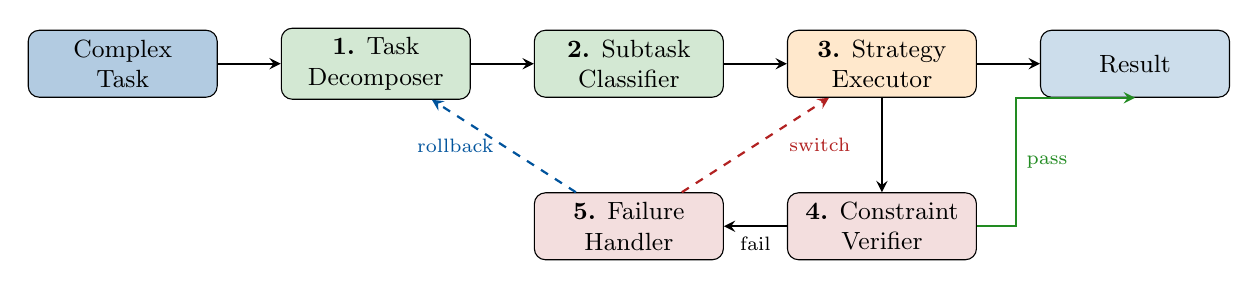
\begin{tikzpicture}[
    node distance=0.8cm,
    block/.style={draw, rounded corners, fill=lightblue, minimum width=2.4cm, minimum height=0.85cm, align=center, font=\small},
    arrow/.style={->, thick, >=stealth}
]
    \node[block, fill=mainblue!30] (input) {Complex\\Task};
    \node[block, fill=successgreen!20, right=of input] (decomp) {\textbf{1.} Task\\Decomposer};
    \node[block, fill=successgreen!20, right=of decomp] (class) {\textbf{2.} Subtask\\Classifier};
    \node[block, fill=warnorange!20, right=of class] (exec) {\textbf{3.} Strategy\\Executor};
    \node[block, fill=mainblue!20, right=of exec] (output) {Result};

    \node[block, fill=alertred!15, below=1.2cm of exec] (verify) {\textbf{4.} Constraint\\Verifier};
    \node[block, fill=alertred!15, below=1.2cm of class] (fail) {\textbf{5.} Failure\\Handler};

    \draw[arrow] (input) -- (decomp);
    \draw[arrow] (decomp) -- (class);
    \draw[arrow] (class) -- (exec);
    \draw[arrow] (exec) -- (output);
    \draw[arrow] (exec) -- (verify);
    \draw[arrow, successgreen] (verify.east) -- ++(0.5,0) |- node[pos=0.25, right, font=\scriptsize] {pass} (output.south);
    \draw[arrow] (verify) -- node[below, font=\scriptsize] {fail} (fail);
    \draw[arrow, dashed, mainblue] (fail) -- node[left, font=\scriptsize] {rollback} (decomp);
    \draw[arrow, dashed, alertred] (fail) -- node[right, font=\scriptsize, xshift=3mm] {switch} (exec);
\end{tikzpicture}

\vspace{0.4cm}
\begin{columns}[T]
\begin{column}{0.45\textwidth}
\small
\textbf{Forward pass:} Decompose $\rightarrow$ Classify $\rightarrow$ Execute
\end{column}
\begin{column}{0.45\textwidth}
\small
\textbf{Recovery loop:} Verify $\rightarrow$ Diagnose $\rightarrow$ Recover
\end{column}
\end{columns}

\end{frame}

\begin{frame}{Module Details (1--3): Decompose, Classify, Execute}

\begin{columns}[T]
\begin{column}{0.48\textwidth}
\textbf{Task Decomposer}
\begin{itemize}
    \item LLM generates hierarchical subtask tree (JSON)
    \item Max depth 3, branching factor 5
    \item \textbf{State-diff prompting}: shows which blocks need to move vs.\ already correct
    \item Re-invoked during rollback with failure diagnostics
\end{itemize}

\vspace{0.2cm}
\textbf{Subtask Classifier}
\begin{itemize}
    \item Labels: spatial, procedural, logical, arithmetic, commonsense
    \item Context-aware: uses parent/sibling info
\end{itemize}
\end{column}

\begin{column}{0.48\textwidth}
\textbf{Strategy Executor}

\vspace{0.1cm}
\small
\begin{tabular}{ll}
\toprule
\textbf{Type} & \textbf{Strategy} \\
\midrule
Spatial & State tracking \\
Procedural & Precondition checking \\
Logical & Tree-of-Thought \\
Arithmetic & Chain-of-Thought \\
Commonsense & Chain-of-Thought \\
\bottomrule
\end{tabular}
\normalsize

\vspace{0.3cm}
On failure, executor receives alternative strategy from fallback ordering per type
\end{column}
\end{columns}

\end{frame}

\begin{frame}{Module Details (4--5): Verify and Recover}

\begin{columns}[T]
\begin{column}{0.48\textwidth}
\textbf{Constraint Verifier}
\begin{itemize}
    \item Deterministic BlocksWorld simulation
    \item Checks preconditions for every action
    \item Checks goal satisfaction at end
    \item No hallucination risk (unlike LLM-based checking)
\end{itemize}

\vspace{0.2cm}
\textbf{Failure Diagnostics}
\begin{itemize}
    \item Classifies error type (blocking dependency, position mismatch, holding conflict, etc.)
    \item Computes \textbf{blocking chains}: ``to unstack A from B, first move C which is on A''
    \item Passed to all recovery tiers
\end{itemize}
\end{column}

\begin{column}{0.48\textwidth}
\textbf{Failure Handler: 4-Tier Recovery}

\vspace{0.2cm}
\begin{enumerate}
    \item \textcolor{successgreen}{\textbf{Strategy switch}} {\small (1 LLM call)} \\
    {\small Re-execute with alternative strategy}

    \vspace{0.15cm}
    \item \textcolor{mainblue}{\textbf{Surgical repair}} {\small (targeted)} \\
    {\small Keep working prefix, fix remaining actions with diagnostic guidance}

    \vspace{0.15cm}
    \item \textcolor{warnorange}{\textbf{Rollback}} {\small (expensive)} \\
    {\small Full re-decomposition from current state with blocking-chain analysis}

    \vspace{0.15cm}
    \item \textcolor{alertred}{\textbf{Propagate}} {\small (give up)} \\
    {\small Report failure after max 3 recovery rounds}
\end{enumerate}
\end{column}
\end{columns}

\end{frame}

% ============================================================
\section{Demo}
% ============================================================

\begin{frame}{Live Demo}

\centering
\vspace{0.5cm}
{\Large Interactive BlocksWorld Planner}

\vspace{0.5cm}
\begin{block}{Demo Features}
\begin{itemize}
    \item Generate tasks with configurable block count (3--10)
    \item Run Our System vs.\ Flat CoT vs.\ ReAct side-by-side
    \item Visual block stacks with step-by-step action playback
    \item Decomposition tree viewer and recovery trace
\end{itemize}
\end{block}

\vspace{0.5cm}
\textbf{Video:} \url{https://youtu.be/s_uiTuxZoVQ}

\end{frame}

% ============================================================
\section{Evaluation}
% ============================================================

\begin{frame}{Experimental Setup}

\begin{columns}[T]
\begin{column}{0.48\textwidth}
\textbf{Benchmark: 60 BlocksWorld tasks}

\vspace{0.2cm}
\begin{tabular}{lcc}
\toprule
\textbf{Level} & \textbf{Blocks} & \textbf{Tasks} \\
\midrule
Easy & 3--4 & 20 \\
Medium & 5--6 & 20 \\
Hard & 7--8 & 20 \\
\bottomrule
\end{tabular}

\vspace{0.3cm}
\begin{itemize}
    \item Fixed random seeds for reproducibility
    \item All methods use GPT-4o
    \item Baselines get 1 attempt (no retries)
\end{itemize}
\end{column}

\begin{column}{0.48\textwidth}
\textbf{Baselines}
\begin{itemize}
    \item \textbf{Flat CoT}: Single-pass step-by-step reasoning
    \item \textbf{Flat ToT}: 3 candidate plans, pick best
    \item \textbf{ReAct}: Interleaved reasoning + acting, up to 15 rounds
\end{itemize}

\vspace{0.3cm}
\textbf{Ablation variants}
\begin{itemize}
    \item Full system
    \item $-$ Classifier
    \item $-$ Adaptive strategy
    \item $-$ Verifier \& Handler
    \item $-$ Failure handler only
    \item Decompose only
\end{itemize}
\end{column}
\end{columns}

\end{frame}

\begin{frame}{Main Results: 82\% Overall (vs.\ 48--70\% Baselines)}

\centering
\begin{tabular}{lcccc}
\toprule
\textbf{Method} & \textbf{Easy} & \textbf{Medium} & \textbf{Hard} & \textbf{Overall} \\
\midrule
Flat CoT & 95\% & 65\% & 50\% & 70\% \\
Flat ToT & 85\% & 40\% & 20\% & 48\% \\
ReAct & 85\% & 65\% & 20\% & 57\% \\
\textbf{Ours (full)} & \textbf{90\%} & \textbf{75\%} & \textbf{80\%} & \textbf{82\%} \\
\bottomrule
\end{tabular}

\vspace{0.5cm}
\begin{columns}[T]
\begin{column}{0.48\textwidth}
\begin{block}{Key Takeaway}
Largest gains on \textbf{hard tasks}: 80\% vs.\ 20--50\%. \\
Pairwise significance: $p < 0.001$ vs.\ ToT, $p < 0.01$ vs.\ ReAct.
\end{block}
\end{column}
\begin{column}{0.48\textwidth}
\begin{block}{Why?}
Easy tasks are simple enough for flat CoT. \\
Hard tasks need decomposition + recovery.
\end{block}
\end{column}
\end{columns}

\end{frame}

\begin{frame}{Scaling: The Gap Widens (9--10 Blocks)}

\begin{columns}[T]
\begin{column}{0.48\textwidth}
\centering
\begin{tabular}{lccc}
\toprule
\textbf{Method} & \textbf{9b} & \textbf{10b} & \textbf{Overall} \\
\midrule
Flat CoT & 20\% & 40\% & 30\% \\
ReAct & 0\% & 0\% & 0\% \\
\textbf{Ours} & \textbf{100\%} & \textbf{80\%} & \textbf{90\%} \\
\bottomrule
\end{tabular}

\vspace{0.4cm}
{\small 20 additional tasks beyond the main benchmark.}
\end{column}

\begin{column}{0.48\textwidth}
\textbf{Why baselines collapse:}
\begin{itemize}
    \item ReAct: 15-round budget exhausted before solving 9--10 block tasks
    \item CoT: one-shot plan almost never correct at this complexity
    \item \textbf{Our system}: decompose into manageable subtasks, recover from errors
\end{itemize}

\vspace{0.2cm}
\begin{block}{Implication}
Hierarchical planning + recovery scales; flat planning does not.
\end{block}
\end{column}
\end{columns}

\end{frame}

\begin{frame}{Ablation Study: What Matters Most?}

\centering
\begin{tabular}{lcccc}
\toprule
\textbf{Variant} & \textbf{Easy} & \textbf{Medium} & \textbf{Hard} & \textbf{Overall} \\
\midrule
Full system & 90\% & 75\% & 80\% & 82\% \\
$-$ Classifier & 90\% & 85\% & 75\% & 83\% \\
$-$ Adaptive strategy & 90\% & 75\% & 75\% & 80\% \\
$-$ Verifier \& Handler & 75\% & 60\% & 35\% & 57\% \\
$-$ Failure handler & 85\% & 65\% & 45\% & 65\% \\
Decompose only & 90\% & 50\% & 35\% & 58\% \\
\bottomrule
\end{tabular}

\vspace{0.4cm}
\begin{columns}[T]
\begin{column}{0.48\textwidth}
\textcolor{alertred}{\textbf{Critical:}} Removing verifier + handler $\rightarrow$ $-$25 points \\
\textcolor{warnorange}{\textbf{Important:}} Removing handler alone $\rightarrow$ $-$17 points
\end{column}
\begin{column}{0.48\textwidth}
\textcolor{mainblue}{\textbf{Supporting:}} Classifier/strategy contribute through recovery, not independently
\end{column}
\end{columns}

\end{frame}

\begin{frame}{Recovery Analysis}

\begin{columns}[T]
\begin{column}{0.48\textwidth}
\textbf{Recovery is the primary differentiator}

\vspace{0.2cm}
\begin{itemize}
    \item 34/60 tasks succeeded on first try (57\%)
    \item 24 tasks triggered recovery
    \item \textbf{15/24 recovered} (63\%)
    \item Without recovery: $\sim$57\% overall \\ (comparable to baselines)
    \item With recovery: 82\% overall
\end{itemize}

\vspace{0.2cm}
\textbf{7 tasks solved \textit{only} by our system} \\
{\small (all baselines failed, all involved recovery)}
\end{column}

\begin{column}{0.48\textwidth}
\textbf{Recovery rate by difficulty}

\vspace{0.2cm}
\begin{tabular}{lc}
\toprule
\textbf{Difficulty} & \textbf{Recovery Rate} \\
\midrule
Easy & 50\% (2/4) \\
Medium & 56\% (5/9) \\
Hard & \textbf{73\% (8/11)} \\
\bottomrule
\end{tabular}

\vspace{0.3cm}
Hard tasks have the \textit{highest} recovery rate --- state-diff prompting and failure diagnostics provide the most actionable guidance on complex tasks.
\end{column}
\end{columns}

\end{frame}

\begin{frame}{Efficiency: Cheaper and Better Than ReAct}

\centering
\begin{tabular}{lcccc}
\toprule
\textbf{Method} & \textbf{Avg Calls} & \textbf{Avg Tokens} & \textbf{Success} & \textbf{Tokens/Success} \\
\midrule
Flat CoT & 1.0 & 394 & 70\% & 563 \\
Flat ToT & 1.0 & 789 & 48\% & 1,633 \\
ReAct & 11.3 & 12,947 & 57\% & 22,848 \\
\textbf{Ours} & \textbf{3.7} & \textbf{3,181} & \textbf{82\%} & \textbf{3,895} \\
\bottomrule
\end{tabular}

\vspace{0.5cm}
\begin{columns}[T]
\begin{column}{0.48\textwidth}
\begin{block}{5.9$\times$ more token-efficient than ReAct}
Targeted calls (decompose, classify, execute) vs.\ 15 iterative rounds
\end{block}
\end{column}
\begin{column}{0.48\textwidth}
\begin{block}{Faster wall-clock time}
8.7s (ours) vs.\ 9.3s (ReAct) --- despite higher success rate
\end{block}
\end{column}
\end{columns}

\end{frame}

% ============================================================
\section{Failure Modes \& Limitations}
% ============================================================

\begin{frame}{Failure Mode Analysis (11/60 Tasks Failed)}

\begin{columns}[T]
\begin{column}{0.48\textwidth}
\textbf{What goes wrong:}

\vspace{0.2cm}
\begin{tabular}{lc}
\toprule
\textbf{Failure Mode} & \textbf{Fraction} \\
\midrule
Cascading recovery errors & 73\% \\
Unknown/edge cases & 18\% \\
Decomposition failures & 9\% \\
\bottomrule
\end{tabular}

\vspace{0.3cm}
\textbf{Dominant mode}: initial plan fails, and each recovery tier introduces its own errors.

\vspace{0.2cm}
\textbf{Failure rate by blocks}: \\
{\small 3b: 0\%, 4b: 17\%, 5b: 12\%, 6b: 33\%, 7b: 25\%, 8b: 12\%}
\end{column}

\begin{column}{0.48\textwidth}
\textbf{Interesting pattern:}

\vspace{0.2cm}
8-block tasks fail \textit{less} (12\%) than 6-block tasks (33\%).

\vspace{0.2cm}
$\rightarrow$ Task \textit{structure} matters more than raw block count.

$\rightarrow$ State-diff prompting helps most on highly structured configurations.

\vspace{0.3cm}
\textbf{Plan quality (successful tasks):}

\vspace{0.1cm}
\begin{tabular}{lc}
\toprule
\textbf{Method} & \textbf{Optimality} \\
\midrule
Baselines & 1.13--1.15$\times$ \\
\textbf{Ours} & \textbf{1.03$\times$} \\
\bottomrule
\end{tabular}

{\small Near-optimal plans from hierarchical structure.}
\end{column}
\end{columns}

\end{frame}

\begin{frame}{Limitations}

\begin{columns}[T]
\begin{column}{0.48\textwidth}
\textbf{Evaluation scope}
\begin{itemize}
    \item Only BlocksWorld --- deterministic, fully observable
    \item 60 tasks (+ 20 scaling) --- moderate sample size
    \item Ours vs.\ CoT not significant at $p < 0.05$ on main benchmark (significant on scaling)
\end{itemize}

\vspace{0.3cm}
\textbf{Domain assumptions}
\begin{itemize}
    \item Deterministic verifier requires known action semantics
    \item Classifier types (spatial, logical, etc.) tuned for planning
    \item Won't directly transfer to open-ended domains
\end{itemize}
\end{column}

\begin{column}{0.48\textwidth}
\textbf{System limitations}
\begin{itemize}
    \item Multiple LLM calls $\rightarrow$ sensitive to API cost/latency
    \item Cascading recovery is the dominant failure mode --- recovery can make things worse
    \item Classifier and adaptive strategy don't independently improve performance
\end{itemize}

\vspace{0.3cm}
\textbf{Reproducibility}
\begin{itemize}
    \item LLM non-determinism causes $\sim$5\% variance across runs
    \item Fixed seeds for task generation, not for LLM sampling
\end{itemize}
\end{column}
\end{columns}

\end{frame}

% ============================================================
\section{Future Work \& Conclusion}
% ============================================================

\begin{frame}{Future Work}

\begin{columns}[T]
\begin{column}{0.48\textwidth}
\textbf{Extending the approach}
\begin{itemize}
    \item Partially observable domains (ALFWorld, household tasks)
    \item Soft constraints and stochastic environments
    \item Probabilistic verifier for non-deterministic actions
\end{itemize}

\vspace{0.3cm}
\textbf{Learning from experience}
\begin{itemize}
    \item Learn decomposition patterns from past successes
    \item Adaptive strategy selection (learned, not rule-based)
    \item Recovery policy: learn which tier to try first
\end{itemize}
\end{column}

\begin{column}{0.48\textwidth}
\textbf{Integration}
\begin{itemize}
    \item Multi-agent collaboration (LangGraph, AutoGen)
    \item Tool use and external knowledge
    \item Grounding in physical environments (robotics)
\end{itemize}

\vspace{0.3cm}
\textbf{Addressing current weaknesses}
\begin{itemize}
    \item Better cascading recovery (meta-reasoning about when to stop)
    \item Reduce over-decomposition on easy tasks
    \item Domain-agnostic verification
\end{itemize}
\end{column}
\end{columns}

\end{frame}

\begin{frame}{Conclusion}

\begin{block}{Summary}
A modular planning system combining \textbf{hierarchical decomposition}, \textbf{adaptive strategy selection}, \textbf{deterministic verification}, and \textbf{tiered failure recovery} for LLM-based agents.
\end{block}

\vspace{0.3cm}
\centering
\begin{tabular}{lcc}
\toprule
& \textbf{Main (60 tasks)} & \textbf{Scaling (20 tasks)} \\
\midrule
Best baseline & 70\% (CoT) & 30\% (CoT) \\
\textbf{Ours} & \textbf{82\%} & \textbf{90\%} \\
\midrule
Hard tasks & 80\% vs.\ 20--50\% & 90\% vs.\ 0--30\% \\
\bottomrule
\end{tabular}

\vspace{0.3cm}
\begin{columns}[T]
\begin{column}{0.45\textwidth}
\small
\textbf{Key finding}: Recovery accounts for 25 percentage points of improvement. 7 tasks solved \textit{only} by our system.
\end{column}
\begin{column}{0.45\textwidth}
\small
\textbf{Efficiency}: 3.7 LLM calls/task, 5.9$\times$ more token-efficient than ReAct, faster wall-clock time.
\end{column}
\end{columns}

\vspace{0.4cm}
\centering
\Large \textcolor{mainblue}{Questions?}

\end{frame}

\end{document}
